\documentclass[11pt,letterpaper]{article}

\usepackage{marvosym}
\usepackage{amsmath,amssymb}
\usepackage[left]{lineno}
\usepackage{changepage}
\usepackage{rotating}
\usepackage{natbib}
\usepackage{setspace}
\usepackage{fancyhdr}
\usepackage{graphicx}
\usepackage{textcomp}
\usepackage{gensymb}
\usepackage{color}
\usepackage{booktabs}
\usepackage{rotating}
\usepackage{longtable}
\usepackage{lscape}
\usepackage{footmisc}
\usepackage{numprint}
\usepackage{siunitx} 
\usepackage{hyperref}
%\doublespacing

%\raggedright
\textwidth = 6.5 in
\textheight = 8.25 in
\oddsidemargin = 0.0 in
\evensidemargin = 0.0 in
\topmargin = 0.0 in
\headheight = 0.0 in
\headsep = 0.2 in
\parskip = 0.1 in
\parindent = 0.1in


\usepackage[aboveskip=1pt,labelfont=bf,labelsep=period,justification=raggedright,singlelinecheck=off]{caption}

\title{Hargraves Magnetometer Quick Start}

\pagestyle{myheadings}
\pagestyle{fancy}
\fancyhf{}
\lhead{Hargraves Magnetometer Quick Start}
\rhead{\thepage}

\begin{document}

\begin{figure}
\vspace*{10pt}
\begin{flushleft}
\textbf{Step 1.}
Open the Visual Basic program (double click the circled icon on the desktop).
\end{flushleft}
\centering
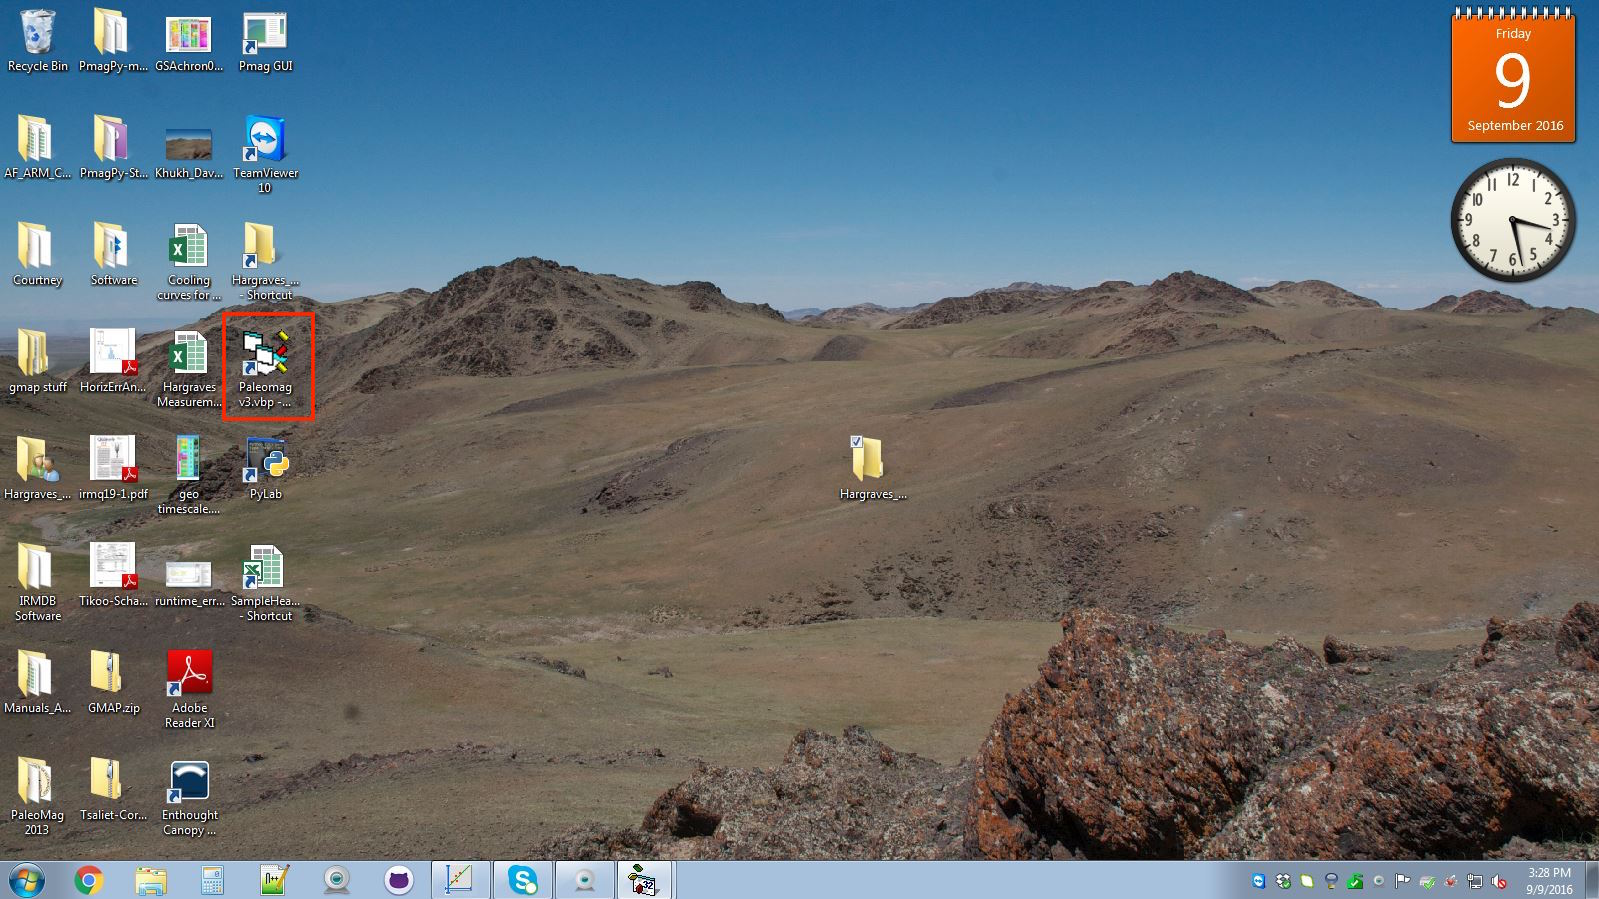
\includegraphics[width=0.9\textwidth]{images/Capture.jpg}
\end{figure}

\begin{figure}
\begin{flushleft}
\textbf{Step 2.}
Press the play icon to open the program interface.
\end{flushleft}
\centering
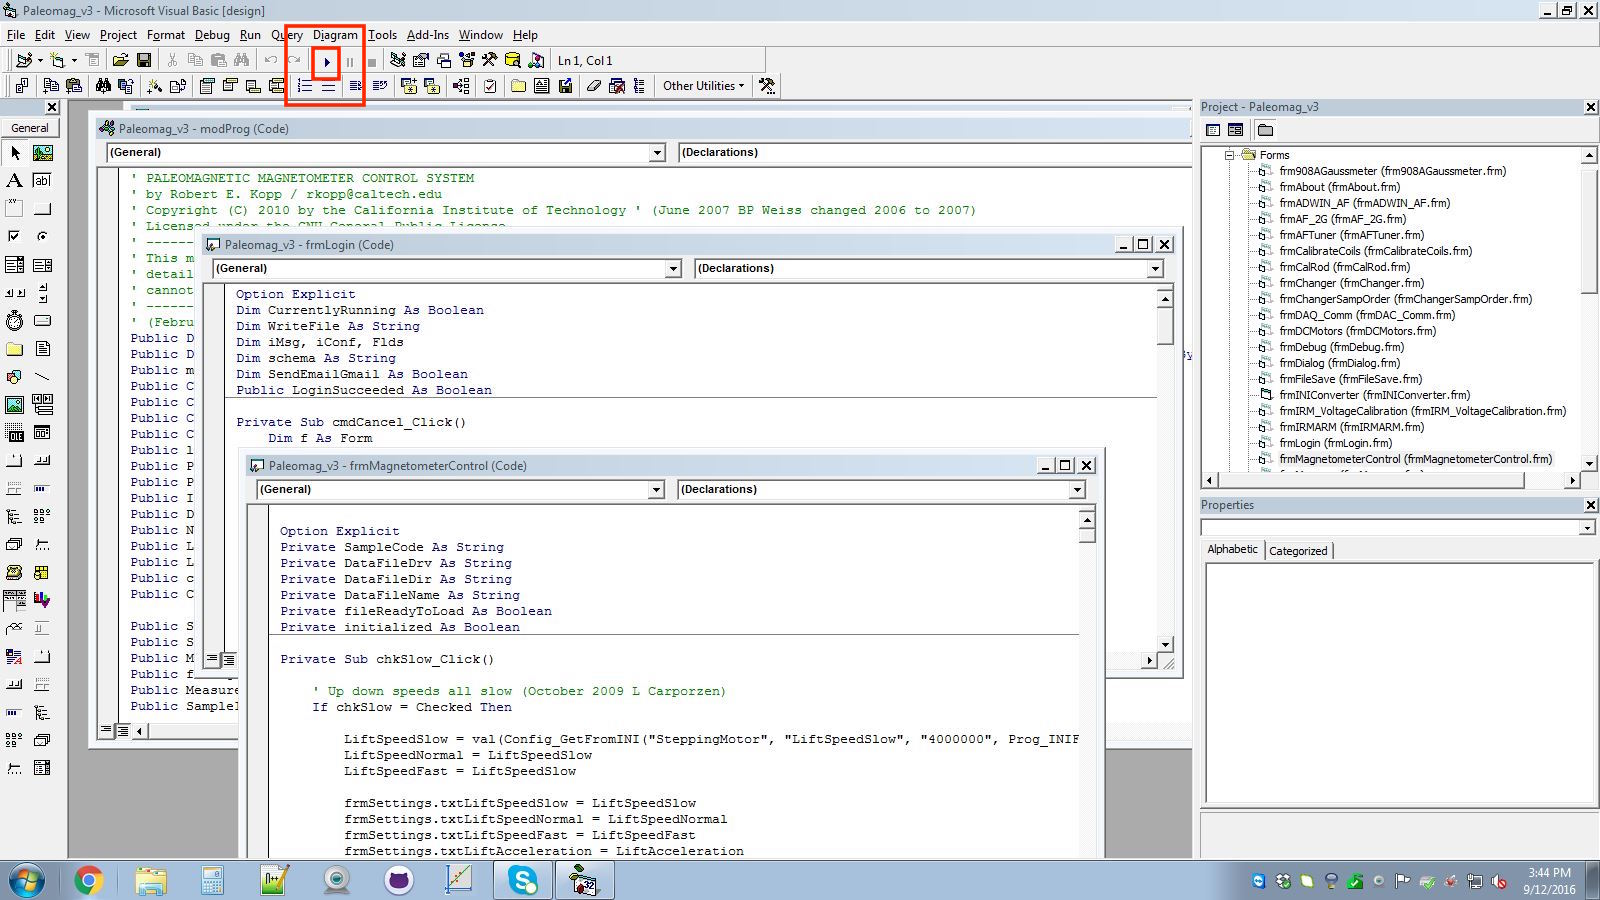
\includegraphics[width=0.9\textwidth]{images/Capture1.jpg}
\end{figure}

\begin{figure}
\begin{flushleft}
\textbf{Step 3.}
Sign in with your name and email.
\end{flushleft}
\centering
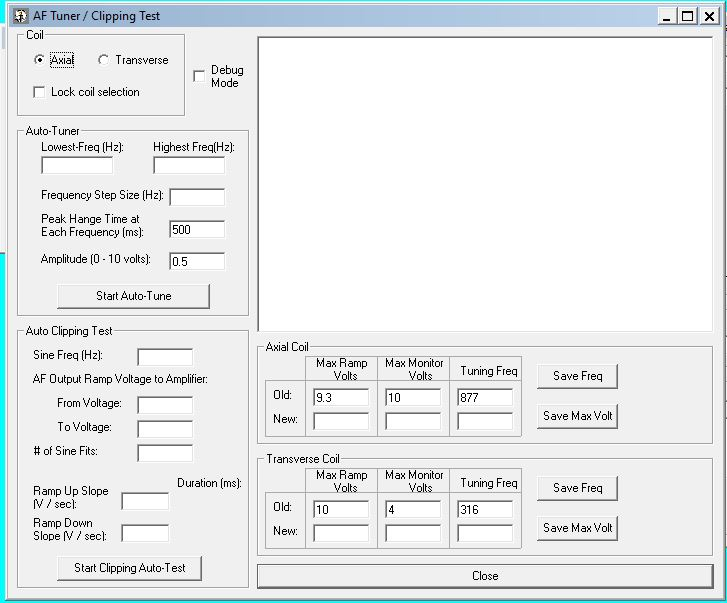
\includegraphics[width=0.9\textwidth]{images/Capture2.jpg}
\end{figure}

\begin{figure}
\begin{flushleft}
\textbf{Step 4.}
The program will ask to home the XY stage to center---you can either choose to do this now (if your samples are already loaded on the tray) or click ``No'' to do it later.
\end{flushleft}
\centering
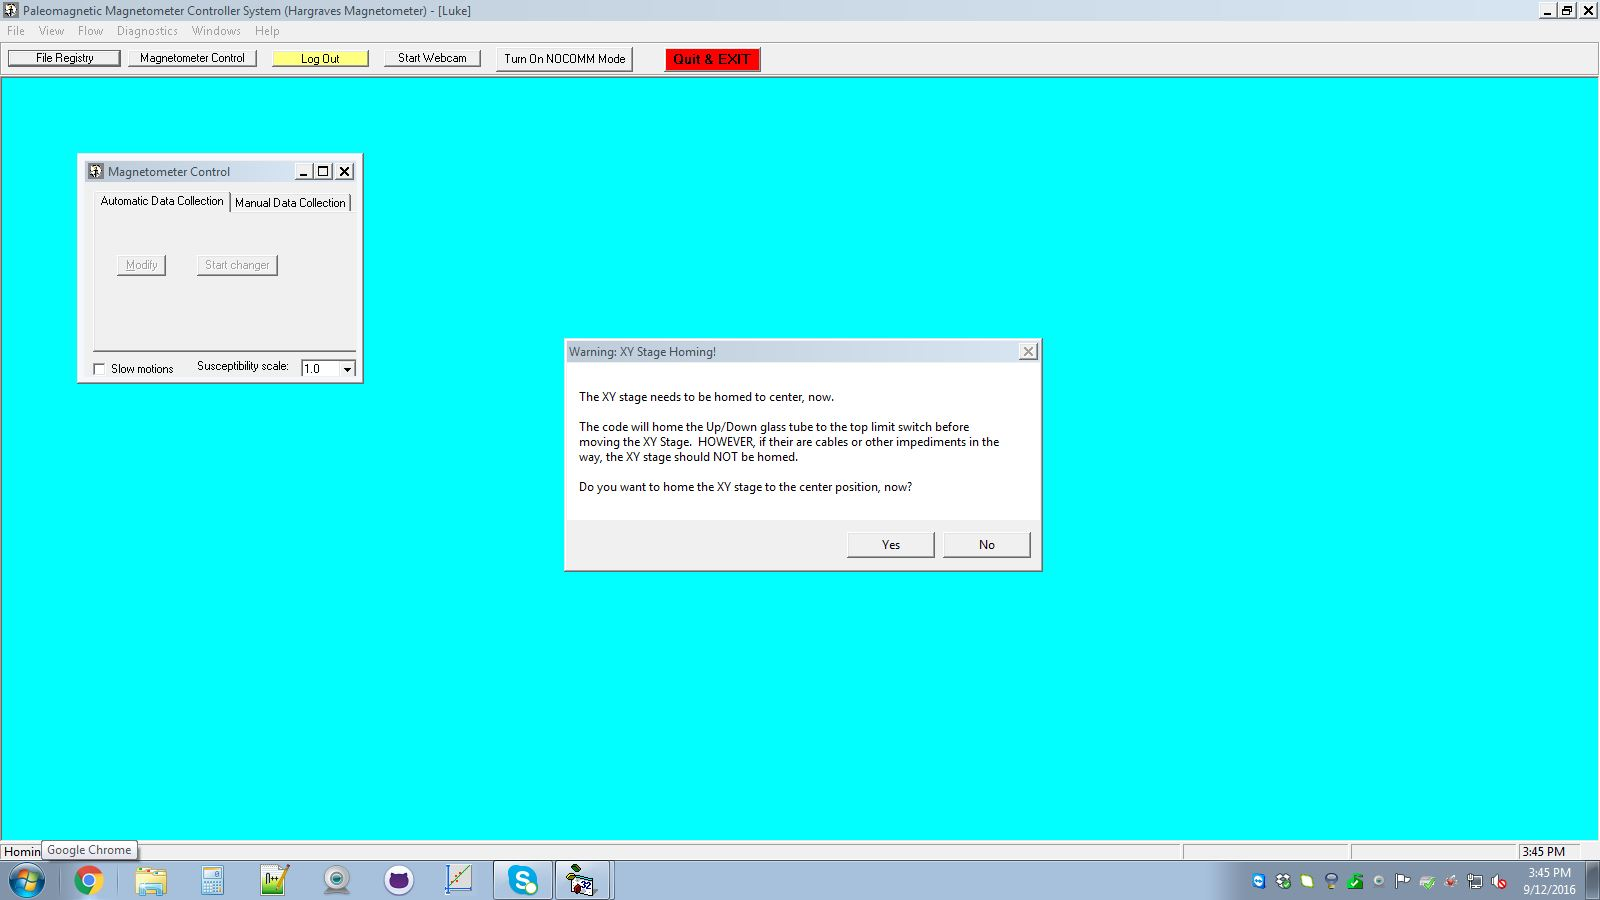
\includegraphics[width=0.9\textwidth]{images/Capture3.jpg}
\end{figure}

\begin{figure}
\begin{flushleft}
\textbf{Step 5.}
The \texttt{Sample Index Registry} window (see below) should open automatically. Click the button marked by the arrow to begin loading your data files into the registry.
\end{flushleft}
\centering
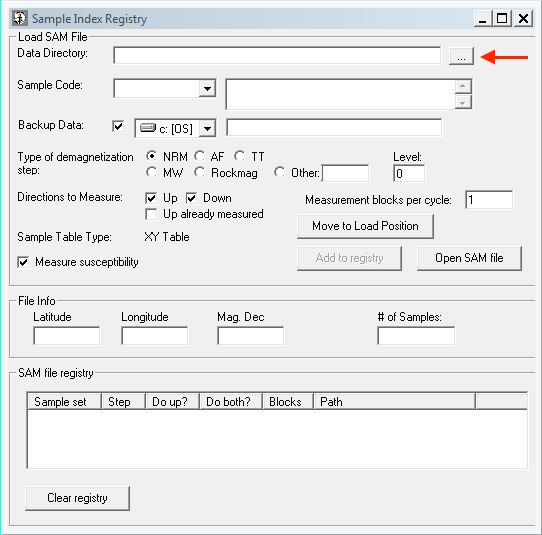
\includegraphics[width=0.9\textwidth]{images/Capture4.jpg}
\end{figure}

\begin{figure}
\begin{flushleft}
\textbf{Step 6.}
In the Hargraves\_Data Dropbox folder, find the SAM file of the first site you want to load.
\end{flushleft}
\centering
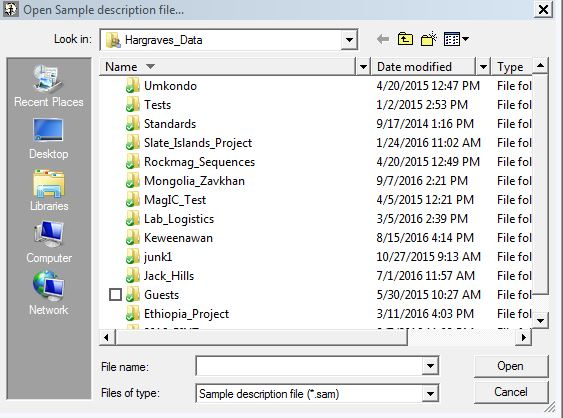
\includegraphics[width=0.9\textwidth]{images/Capture5.jpg}
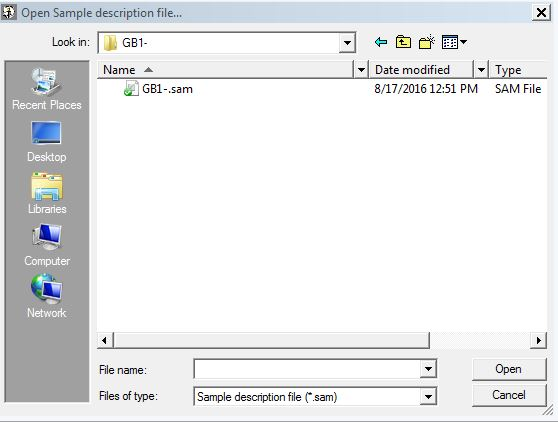
\includegraphics[width=0.9\textwidth]{images/Capture6.jpg}
\end{figure}

\begin{figure}
\begin{flushleft}
\textbf{Step 7.}
\begin{enumerate}
\item{Uncheck ``Backup Data''.} 
\item{Specify the treatment step of the samples you are measuring. In the example below, samples have been thermally demagnetized (``TT'') to 200 \textdegree C.}
\item{Specify the orientations of samples you wish to measure. Both ``Up'' and ``Down'' should be measured when possible. If ``Up'' directions were measured previously and you are only measuring ``Down'', uncheck ``Up'' and check ``Up already measured''.}
\item{Specify whether you want to measure susceptibility}.
\item{Add the site to the registry.}
\end{enumerate}
\end{flushleft}
\centering
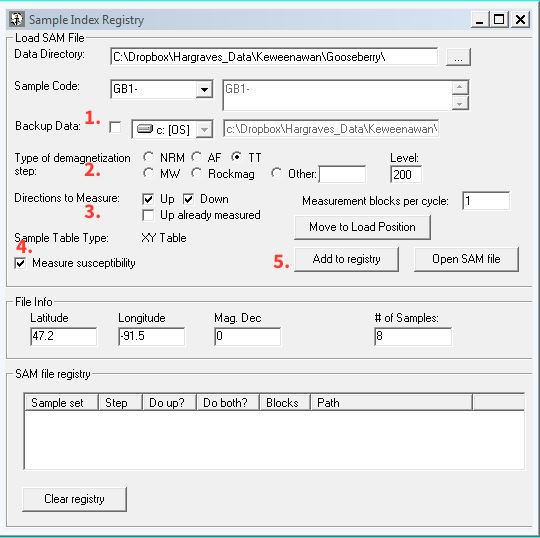
\includegraphics[width=0.9\textwidth]{images/Capture7.jpg}
\end{figure}

\begin{figure}
\begin{flushleft}
\textbf{Step 8.}
Repeat step 7 for all sites and fill the registry.
\end{flushleft}
\centering
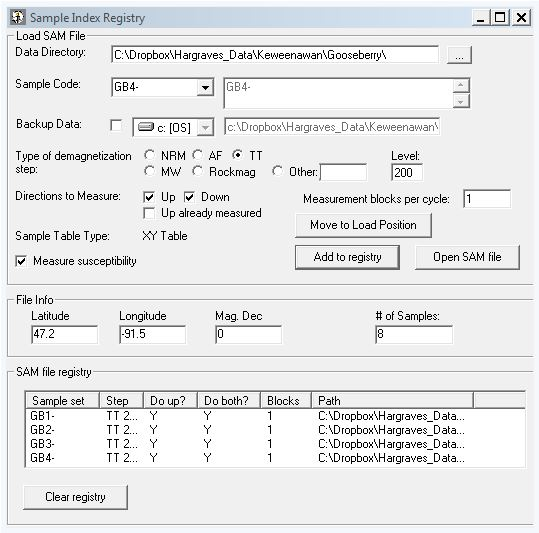
\includegraphics[width=0.6\textwidth]{images/Capture8.jpg}
\end{figure}

\begin{figure}
\begin{flushleft}
\textbf{Step 9.}
In the \texttt{Magnetometer Control} window, click ``Modify''.
\end{flushleft}
\centering
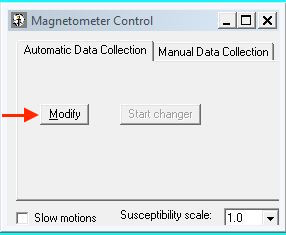
\includegraphics[width=0.6\textwidth]{images/Capture9.jpg}
\end{figure}

\begin{figure}
\begin{flushleft}
\textbf{Step 10.}
Specify the position (hole number) of the first sample. Click ``Add to list''. This will assign positions on the tray for all the samples in the registry in the order that they were loaded (starting from the initial position). Click ``View new sample list'' and check that the positions of the samples on the tray are correct. 
\end{flushleft}
\centering
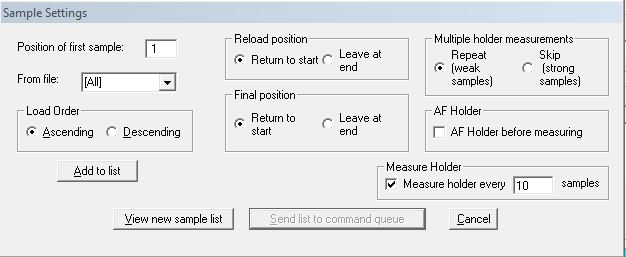
\includegraphics[width=0.9\textwidth]{images/Capture10.jpg}
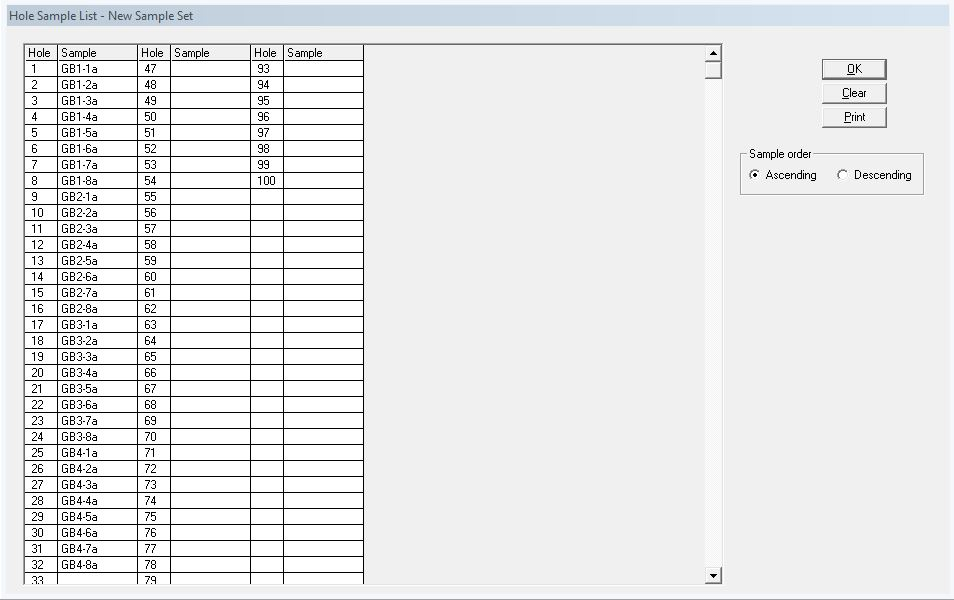
\includegraphics[width=\textwidth]{images/Capture11.jpg}
\end{figure}

\begin{figure}
\begin{flushleft}
\textbf{Step 11.}
If you chose not to home the XY stage in Step 4, the system will ask you to do this now. If you have started the program from scratch (i.e. you did not simply log off a different user and log back in), the system will confirm the position of the glass holder once the XY stage homes to center. Check to make sure the glass holder is positioned over the hole in the tray (cup number 46). If it is, enter 46 and click Okay. If it isn't, something is wrong. 
\end{flushleft}
\centering
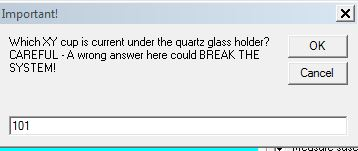
\includegraphics[width=0.7\textwidth]{images/Capture12.jpg}
\end{figure}

\begin{figure}
\begin{flushleft}
\textbf{Step 11.}
Click ``Start changer'' to begin your measurements!
\end{flushleft}
\centering
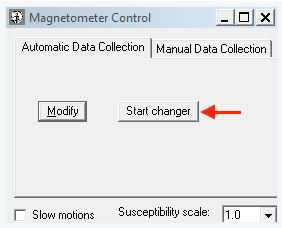
\includegraphics[width=0.7\textwidth]{images/Capture13.jpg}
\end{figure}

\clearpage

\section*{Miscellaneous Tips}
\subsection*{SQuID jumps}
The occassional SQuID jump is not a cause for concern---the magnetometer will remeasure samples up to three times before giving up (you will receive an email notification for this). For some samples, however, frequent SQuID jumps might be more of a nuisance, especially if multiple automatic remeasurements by the magnetometer don't seem to be resolving the issue. SQuID jumps may be improved or eliminated by slowing down the up/down and turning motors. This slows down the measurement process and decreases the chance of a flux jump for strongly magnetic samples.

In the program window, go to \textsf{View}$\rightarrow$\textsf{Settings}. Under the \textsf{DC Motors (1)} tab, lower the \textsf{Lift speed slow} and \textsf{Turning speed} values. To maintain reasonable operating speeds, do not decrease the values to a lower magnitude. For example, start by lowering \textsf{Lift speed slow} from $3\times10^7$ to $2\times10^7$ and see if the SQuID jumps improve.

\subsection*{Sample gets stuck on descent}
If you receive an ``unacceptable slop'' notification, it is most likely due to a sample that has been caught on the edge of the tray as it is being lowered into the magnetomter. Go to \textsf{Diagnostics}$\rightarrow$\textsf{DC Motors} and click \textsf{Home to Top}. Unless it has dropped through the magnetometer, quickly adjust the sample on the holder before it descends again. Be sure to ``Resume'' the run.

%the following tip leads to other problems with the file and should not be followed
%\subsection*{The multiple-site ``flip'' glitch}
%If you are measuring many sites on the same tray, a glitch in the program causes a separate ``flip samples'' notification (and corresponding holder measurement) for each site after you flip your samples. If you are measuring very many sites on the same tray and want to save time, after flipping your samples go to \textsf{View}$\rightarrow$\textsf{Command Queue} and delete the multiple ``flip'' and ``holder measurement'' commands before the first sample measurement (make sure to leave one of the ``holder measurement'' commands).



\end{document}
